\documentclass{beamer}
\usetheme{Hannover}


\usepackage{algorithm}
\usepackage{algorithmic}
\usepackage{amsmath}
\usepackage{amssymb}
\usepackage{amsthm}
\usepackage[ngerman,english]{babel}
\usepackage{centernot} 
\usepackage{color}
\usepackage{dsfont}
\usepackage{graphicx}
\usepackage[utf8]{inputenc}
\usepackage{import}
\usepackage{standalone}
\usepackage{qtree}

\usepackage{hyperref}

\title{Integral infeasibility and testing total dual integrality}
\author{David L.Applegate, William Cook S.Thomas McCormick}

\newcommand{\N}{\ensuremath{\mathds{N}}}
\newcommand{\R}{\ensuremath{\mathds{R}}}
\newcommand{\red}[1]{\textcolor{red}{#1}}

\setlength{\itemsep}{-2pt}


\begin{document}

\begin{frame}{Example}
	\begin{enumerate}
		\pause
		\item Item 1:\\
		 $\mathcal{O}(log(n))$ explanation
		\pause
		\item Item 2 
	\end{enumerate}
\end{frame}

%%%%%%%%%%%%%%%%%%
%%%%%%    %%%%%%%%
%%%%%%%%%%%%%%%%%%

% RB-Tree Eigenschaften

\begin{frame}

	\begin{block}{Red-Black Tree (RB Tree) Properties}
		\begin{enumerate}
			\small
			\item <2-> 1
			\item <3-> 2
			\item <4-> 3
			\item <5-> 4
			\item <6-> 5
		\end{enumerate}
	\end{block}
\end{frame}

%%%%%%%%%%%%%%%%%%
%%%%%%    %%%%%%%%
%%%%%%%%%%%%%%%%%%

\begin{frame}
	\frametitle{Example}
	
	% Beispiel RB Tree
	\begin{figure}[htp]
		\centering
		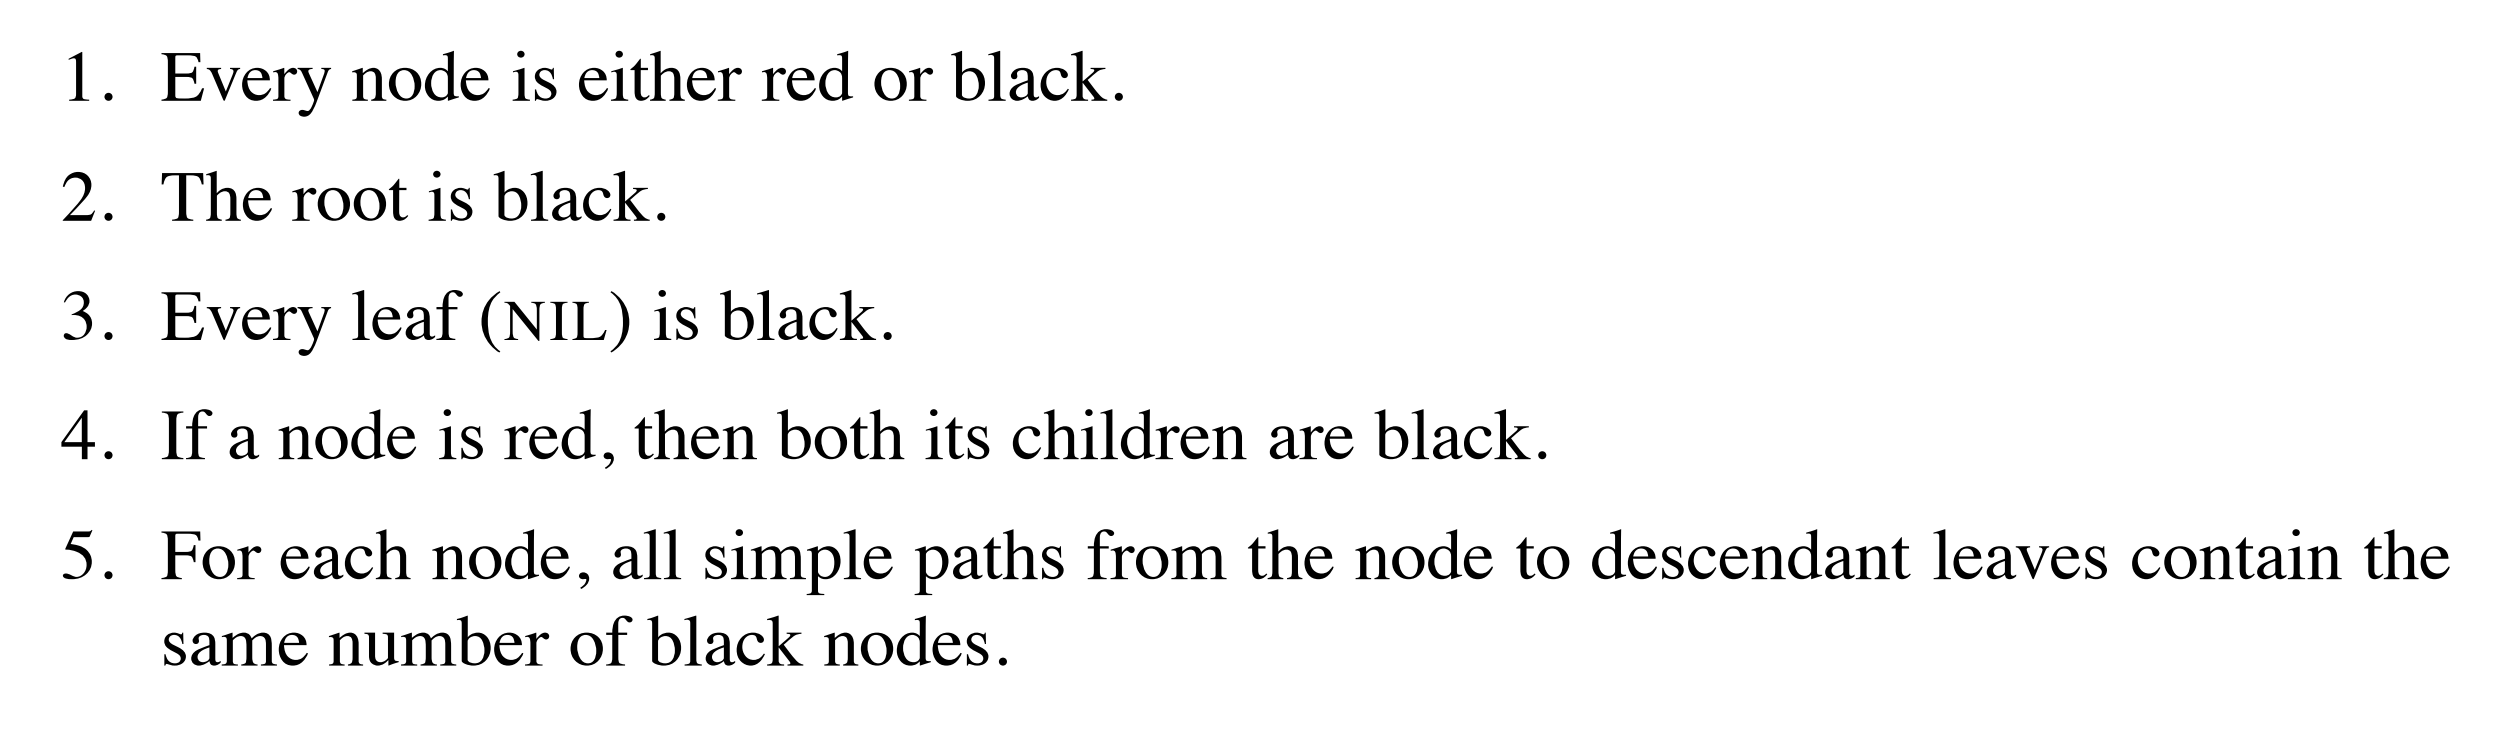
\includegraphics[width=10cm]{images/example.png}
		\caption{Example Image}
		\label{fig:something}
	\end{figure}
\end{frame}

\begin{frame}
	\frametitle{Introduction of the problem}
	Let $s$ be a rational linear system $Ax \leqslant b$\\
	$s$ is called totally dual integral if :
 
	$\forall \text{integral vector }w$ such that there is an optima for the following equation $max\{wx:Ax\leqslant b\}=min\{yb:yA=w,y\geqslant 0\}$, there is an integral solution tothe minimum equation. If $b$ is integral aswell, there is also an inegral solution for the maximum in the equation.

\end{frame}

\begin{frame}
	\frametitle{Goals}
	\begin{enumerate}
		\item 
\end{document}

